
\documentclass{InsightArticle}

\usepackage[dvips]{graphicx}
\usepackage{color}
\usepackage{listings}					%List program code source

\definecolor{listcomment}{rgb}{0.0,0.5,0.0}
\definecolor{listkeyword}{rgb}{0.0,0.0,0.5}
\definecolor{listnumbers}{gray}{0.65}
\definecolor{listlightgray}{gray}{0.955}
\definecolor{listwhite}{gray}{1.0}


%%%%%%%%%%%%%%%%%%%%%%%%%%%%%%%%%%%%%%%%%%%%%%%%%%%%%%%%%%%%%%%%%%
%
%  hyperref should be the last package to be loaded.
%
%%%%%%%%%%%%%%%%%%%%%%%%%%%%%%%%%%%%%%%%%%%%%%%%%%%%%%%%%%%%%%%%%%
\usepackage[dvips,
bookmarks,
bookmarksopen,
backref,
colorlinks,linkcolor={blue},citecolor={blue},urlcolor={blue},
]{hyperref}


\title{STL file format MeshIO class for ITK}

%
% NOTE: This is the last number of the "handle" URL that
% The Insight Journal assigns to your paper as part of the
% submission process. Please replace the number "1338" with
% the actual handle number that you get assigned.
%
\newcommand{\IJhandlerIDnumber}{1338}

% Increment the release number whenever significant changes are made.
% The author and/or editor can define 'significant' however they like.
\release{1.00}

% At minimum, give your name and an email address.  You can include a
% snail-mail address if you like.
\author{Luis Ibanez$^{1}$}
\authoraddress{$^{1}$Kitware Inc. Clifton Park, NY}

\begin{document}

%
% Add hyperlink to the web location and license of the paper.
% The argument of this command is the handler identifier given
% by the Insight Journal to this paper.
%
\IJhandlefooter{\IJhandlerIDnumber}


% Setup source code listings
\lstset{frame = tb,
       framerule = 0.25pt,
       float,
       fontadjust,
       backgroundcolor={\color{listlightgray}},
       basicstyle = {\ttfamily\footnotesize},
       keywordstyle = {\ttfamily\color{listkeyword}\textbf},
       identifierstyle = {\ttfamily},
       commentstyle = {\ttfamily\color{listcomment}\textit},
       stringstyle = {\ttfamily},
       showstringspaces = false,
       showtabs = false,
       numbers = left,
       numbersep = 6pt,
       numberstyle={\ttfamily\color{listnumbers}},
       tabsize = 2,
       language=[ANSI]C++,
       floatplacement=!h
       }


\ifpdf
\else
   %
   % Commands for including Graphics when using latex
   %
   \DeclareGraphicsExtensions{.eps,.jpg,.gif,.tiff,.bmp,.png}
   \DeclareGraphicsRule{.jpg}{eps}{.jpg.bb}{`convert #1 eps:-}
   \DeclareGraphicsRule{.gif}{eps}{.gif.bb}{`convert #1 eps:-}
   \DeclareGraphicsRule{.tiff}{eps}{.tiff.bb}{`convert #1 eps:-}
   \DeclareGraphicsRule{.bmp}{eps}{.bmp.bb}{`convert #1 eps:-}
   \DeclareGraphicsRule{.png}{eps}{.png.bb}{`convert #1 eps:-}
\fi


\maketitle


\ifhtml
\chapter*{Front Matter\label{front}}
\fi


% The abstract should be a paragraph or two long, and describe the
% scope of the document.
\begin{abstract}
\noindent
This document describes the implementation of an ITK class to support the
reading and writing of Meshes in STL file format. The Meshes are assumed to
contain 2D manifolds embedded in a 3D space. In practice, it would be desirable
to use this class mostly to read and write QuadEdgeMeshes.

This paper is accompanied with the source code, input data, parameters and
output data that the authors used for validating the algorithm described in
this paper. This adheres to the fundamental principle that scientific
publications must facilitate reproducibility of the reported results.

\end{abstract}

\IJhandlenote{\IJhandlerIDnumber}

\tableofcontents

\section{Introduction}

The STL file format is a very common standards for the transmission of Mesh
data.  Originally designed for Stereo Lithography, the STL format has become a
widely used standard for storing and sharing mesh data.

\begin{center}
\url{http://en.wikipedia.org/wiki/STL_(file_format)}
\end{center}

In recent years, the STL file format has been adopted as the standard way of
preparing shapes as input to 3D printing. Given that ITK is a natural choice
for segmenting anatomical structures from 3D medical data, it is desirable to
be able to generate meshes from such structures, and then store them in STL
files suitable for 3D printing. The class described in this article will make
that possible, using a pure ITK pipeline.


\section{Software Requirements}

You need to have the following software installed:

% The {itemize} environment uses a bullet for each \item.  If you want the 
% \item's numbered, use the {enumerate} environment instead.
\begin{itemize}
  \item  Insight Toolkit 4.5
  \item  CMake 2.8
\end{itemize}

For convenience, the code has been configured as an External module. This means
that you can

\begin{itemize}
\item Take the source tree of this article
\item Copy it into the ITK/Modules/External directory
\item Reconfigure ITK with CMake
\item Compile
\item Start using the new STLMeshIO class for reading and writing
\end{itemize}

The External modules in ITK facilitate the process of adding customized classes
to the toolkit in local installations~\cite{Liu2013}.

\section{Infrastructure}

This STLMeshIO class build upon the infrastructure of the classes

\begin{itemize}
\item MeshIOBase
\item MeshFileReader
\item MeshFileWriter
\end{itemize}

and uses the IO factory mechanism.

Therefore, we register the STLMeshIOFactory class as an available provider of
MeshIO classes, and with this, depending on the filenames (particularly the
filename extension) that are requested for reading or writing, this specific
MeshIO class may be internally selected for the task by ITK.

For more details on the Mesh IO Framework, please see this
article~\cite{Zhu2010}:

\begin{itemize}
\item \url{http://www.insight-journal.org/browse/publication/761}
\item \url{http://hdl.handle.net/10380/3212}
\end{itemize}


\section{How to Use}

The following code example illustrates how to use the STLMeshIO class to read and write Meshes.

We start with including the headers of fundamental classes:

\begin{center}
\lstset{firstnumber=19}
\lstinputlisting[linerange={19-23}]{../../Source/ITKSTLMeshIO/test/itkSTLMeshIOTest.cxx}
\end{center}


We declare the type of the new Mesh.

\begin{center}
\lstset{firstnumber=35}
\lstinputlisting[linerange={35-38}]{../../Source/ITKSTLMeshIO/test/itkSTLMeshIOTest.cxx}
\end{center}

The QuadEdgeMeshe is probably the best type of Mesh to use to host the content
of STL files, given that it represents a 2D surface embedded into a 3D space.

We register the STLMeshIO factory in the Mesh IO framework with the line:

\begin{center}
\lstset{firstnumber=40}
\lstinputlisting[linerange={40-40}]{../../Source/ITKSTLMeshIO/test/itkSTLMeshIOTest.cxx}
\end{center}

The STL MeshIO class will respond to requests for reading or writing any mesh whose filename uses the extensions

\begin{itemize}
\item .stl
\item .STL
\end{itemize}

The factory framework will take care of selecting the appropriate MeshIO class.

We can now declare and instantiate a MeshFileReader and a MeshFileWriter

\begin{center}
\lstset{firstnumber=42}
\lstinputlisting[linerange={42-46}]{../../Source/ITKSTLMeshIO/test/itkSTLMeshIOTest.cxx}
\end{center}

Set the filenames to be read and to be written

\begin{center}
\lstset{firstnumber=48}
\lstinputlisting[linerange={48-49}]{../../Source/ITKSTLMeshIO/test/itkSTLMeshIOTest.cxx}
\end{center}

Select whether we are going to write out an STL file in ASCII or BINARY format

\begin{center}
\lstset{firstnumber=51}
\lstinputlisting[linerange={51-60}]{../../Source/ITKSTLMeshIO/test/itkSTLMeshIOTest.cxx}
\end{center}

In this particular example, we connect them together

\begin{center}
\lstset{firstnumber=69}
\lstinputlisting[linerange={69-69}]{../../Source/ITKSTLMeshIO/test/itkSTLMeshIOTest.cxx}
\end{center}

and trigger the reading and writing by calling the Update() method in the writer

\begin{center}
\lstset{firstnumber=73}
\lstinputlisting[linerange={73-81}]{../../Source/ITKSTLMeshIO/test/itkSTLMeshIOTest.cxx}
\end{center}


\section{Examples}

STL files can use either an ASCII representation or a BINARY representation.

\subsection{ASCII}

The ASCII representation follows the structure:

\begin{lstlisting}
solid ascii
 facet normal nx ny nz
  outer loop
   vertex x1 y1 z1
   vertex x2 y2 z2
   vertex x3 y3 z3
  endloop
 endfacet
 ...
 [next facet]
 ...
endsolid
\end{lstlisting}

\begin{center}
\url{http://en.wikipedia.org/wiki/STL_(file_format)#ASCII_STL}
\end{center}

\subsection{BINARY}

The BINARY representation follows the structure:

\begin{lstlisting}
UINT8[80] – Header
UINT32 – Number of triangles

foreach triangle
REAL32[3] – Normal vector
REAL32[3] – Vertex 1
REAL32[3] – Vertex 2
REAL32[3] – Vertex 3
UINT16 – Attribute byte count
end
\end{lstlisting}

\begin{center}
\url{http://en.wikipedia.org/wiki/STL_(file_format)#Binary_STL}
\end{center}

\subsection{Screenshots}


\begin{figure}[!htb]
\centering
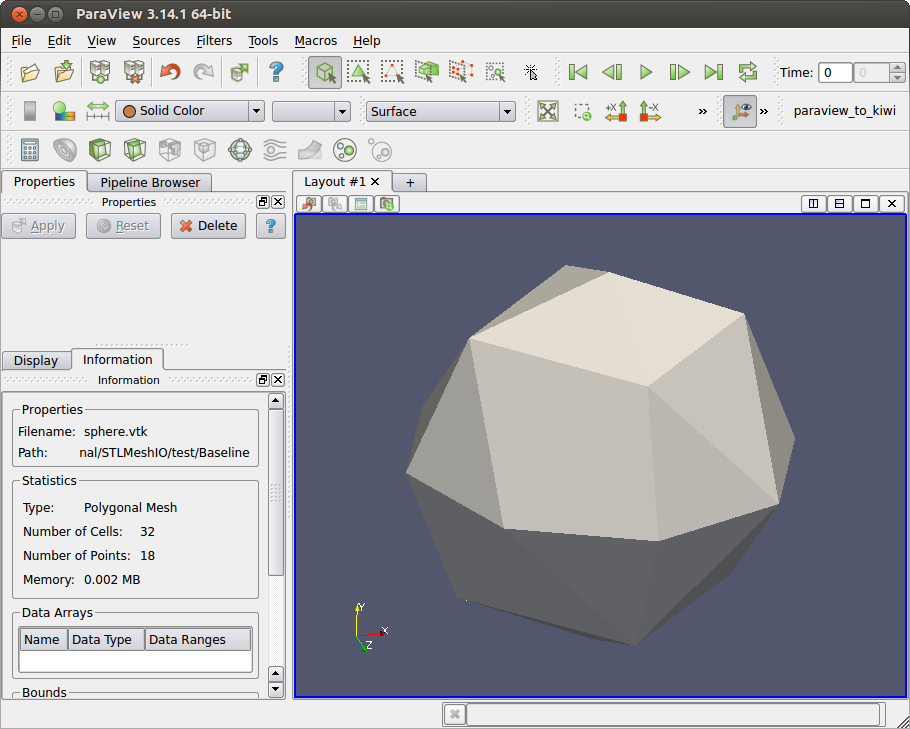
\includegraphics[width=\textwidth]{SphereInParaviewVTK.eps}
\caption{Input Sphere in VTK format displayed in Paraview}
\end{figure}


\begin{figure}[!htb]
\centering
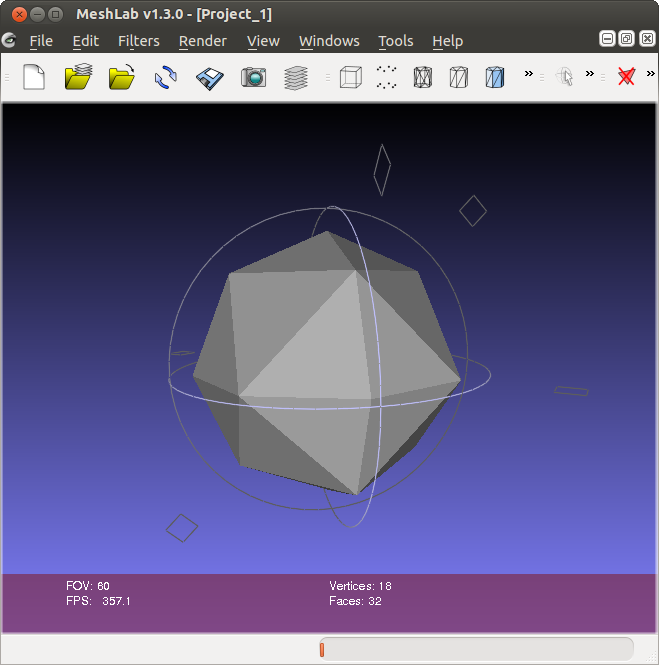
\includegraphics[width=\textwidth]{SphereInMeshLabSTL.eps}
\caption{Output Sphere in STL format displayed in Meshlab}
\end{figure}


\section{Conclusion}

It should now be possible to use the STL MeshIO class to write out directly
from ITK the segmentations of anatomical structures, and feed them into a 3D
printing pipeline.



%%%%%%%%%%%%%%%%%%%%%%%%%%%%%%%%%%%%%%%%%
%
%  Insert the bibliography using BibTeX
%
%%%%%%%%%%%%%%%%%%%%%%%%%%%%%%%%%%%%%%%%%

\bibliographystyle{plain}
\bibliography{InsightJournal}

\end{document}
